% Qualitative schematic of the source diagram; geometry is not to scale.
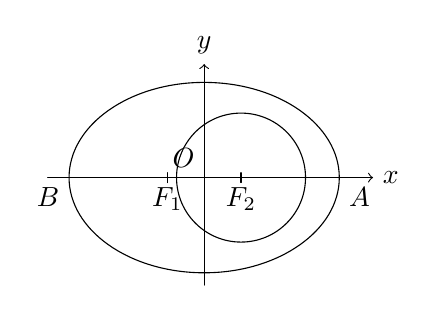
\begin{tikzpicture}[line cap=round,line join=round,scale=0.78]
  \coordinate (O) at (0,0);
  \coordinate (Fone) at (-0.6,0);
  \coordinate (Ftwo) at (0.6,0);
  \coordinate (A) at (2.2,0);
  \coordinate (B) at (-2.2,0);

  % Axes and the elliptical orbit.  No unprovided distances are asserted.
  \draw[->] (-2.55,0)--(2.75,0) node[right] {$x$};
  \draw[->] (0,-1.75)--(0,1.85) node[above] {$y$};
  \draw (O) ellipse (2.2 and 1.55);
  % The source depicts the Earth circle centered at F_2 and enclosing O.
  \draw (Ftwo) circle[radius=1.05];

  % Foci are shown as short axis ticks, as in the source.
  \draw (-0.6,-0.08)--(-0.6,0.08);
  \draw (0.6,-0.08)--(0.6,0.08);
  \node[above left] at (O) {$O$};
  \node[below] at (Fone) {$F_1$};
  \node[below] at (Ftwo) {$F_2$};
  \node[below right] at (A) {$A$};
  \node[below left] at (B) {$B$};
\end{tikzpicture}
